\documentclass{article}
\usepackage{qilin}
\tikzstyle{process} = [rectangle, rounded corners, minimum width=1.5cm, minimum height=0.5cm,align=center, draw=black, fill=gray!30, auto]
\title{PHY460: Nonlinear Physics}
\author{QiLin Xue}
\date{Fall 2022}
\usepackage{mathrsfs}
\usetikzlibrary{arrows}
\usepackage{stmaryrd}
\usepackage{accents}
\newcommand{\ubar}[1]{\underaccent{\bar}{#1}}
\usepackage{pgfplots}
\numberwithin{equation}{section}

\begin{document}

\maketitle
\tableofcontents
\newpage
\section{Introduction}
Given some $\dot{\vec{x}}=\vec{v}(x),$ where $x$ is some generalized coordinate, then starting from $x_0$ at $t=0,$ trajectories are locally linear, given sufficiently smooth $\vec{v}(x)$ and sufficiently small $t.$

\emf{Fixed points} are when that velocity field is zero. Fixed points can either be stable, unstable, or semi-stable, and can be analyzed by either taking derivatives or looking at the phase portrait at that point. For example, consider $\dot{x}=\sin x,$ then
\begin{center}
    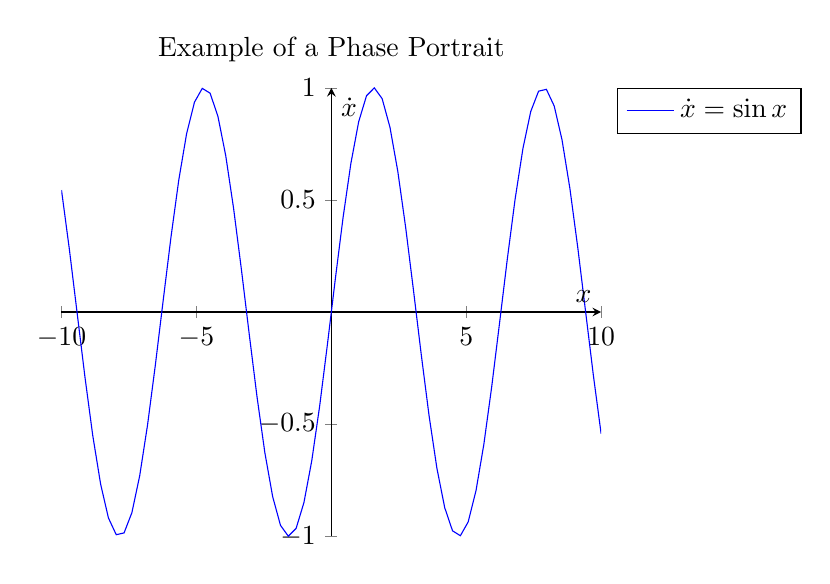
\begin{tikzpicture}
    \begin{axis}[
    legend pos=outer north east,
    title=Example of a Phase Portrait,
    axis lines = middle,
    xlabel = $x$,
    ylabel = $\dot{x}$,
    variable = t,
    trig format plots = rad,
    ]
    \addplot [
        domain=-10:10,
        samples=70,
        color=blue,
        ]
        {sin(x)};
    \addlegendentry{$\dot{x}=\sin x$}
    \end{axis}
    \end{tikzpicture}
\end{center}
While $x=\pi$ is a stable stationary point, it is not immediately clear that a particle will actually reach this point. To properly analyze it, we need to integrate the equation.

Take $f(x_0)=0,$ where $x_0$ is a fixed point. Recall that 
\begin{equation*}
    f(x) = f(x_0) + (x-x_0) + (x-x_0)f'(x_0) + \frac{1}{2}(x-x_0)^2f''(x_0) + \frac{1}{3!}(x-x_0)^3 f'''(x_0)\cdots
\end{equation*}
First assume that $f'(x_0) \neq 0,$ so we only need to keep this first term. Our ODE takes the form of 
\begin{equation*}
    \frac{d(x-x_0)}{dt} = f'(x_0)(x-x_0), 
\end{equation*}
where the solution is 
\begin{equation*}
    x(t)-x_0 = e^{f'(x_0)t}(x(0)-x_0).
\end{equation*}
We look at cases:
\begin{itemize}
    \item Case 1: $f'(x_0) > 0.$ If $x(0)>x_0,$ it flows away as $t$ increases. If $x(0)<x_0,$ it also flows away as $t$ increases. The position grows initially as $e^{f'(x_0)t}$, with $e^{f'(x_0)t} > 1 \forall t >0.$
    \item Case 2: $f'(x_0) < 0.$ The converse is true
    \item Special case where $f'(x_0) = 0$ but $f''(x_0) \neq 0.$ This gives a semi-stable behavior governed by $f''(x_0).$
\end{itemize}
\begin{example}
    We look at an interesting example of $\dot{x} = x^{1/3},$ such that the acceleration scales as $v'(x) = x^{-2/3},$ which diverges as $x\to 0.$
    \vspace{2mm}

    There are actually an infinite amount of solutions. Existence and uniqueness theorems will require that both $f(x)$ and $f'(x)$ exist in some small open interval around $x_0.$
\end{example}
\begin{theorem}
    Existence and Uniqueness of Solutions: Consider the 1D case of $\dot{x} = v(x).$ E\&U stipulates that $\dot{x} = v(x)$ has a unique solution around the initial condition $(t_0,x_0)$ provided the functions are smooth in the sense of the \emf{Lipschitz condition.}
\end{theorem}
\begin{definition}
    $v(x)$ is smooth for $x \in (a,b)$ if $v(x)$ is continuous and differentiable in $(a,b).$ The $\dot{v}(x)$ can be discontinuous.
    \vspace{2mm}
\end{definition}
Recall that continuity means that for all $x,y\in (a,b),$ then there exists some $K$ such that $|v(x)-v(y)| < K|x-y|,$ so a finite derivative exists almost everywhere. Differentiability means that for all $x,y\in (a,b),$ then there exists some $K$ such that $|v(x)-v(y)| < K|x-y|^2,$ so a finite second derivative exists almost everywhere. The Lipschitz condition is that for all $x,y\in (a,b),$ then there exists some $K$ such that $|v(x)-v(y)| < K|x-y|^p,$ so a finite $p$ derivative exists almost everywhere.

Our systems, if they meet the Lipschitz condition, have a solution beginning at $t_0$ for all $x_0 \in (a,b).$ All solutions of $\dot{x} = v(x)$ starting at $x_0,t_0$ are the same for some amount of time.

This solution can be found explicitly using \emf{Barron's Formula,} which states that for $\dot{x} = v(x),$ then 
\begin{equation*}
    t-t_0 = \int_{-x_0}^{\varphi(t)} \frac{dx}{v(x),}
\end{equation*}
where $\varphi(t)=x(t)$ is the final position.

\textit{Some comments on E\&U:} Imagine at some $x_0,$ we have $v(x_0)=0.$ We start at $x_0$ at $t_0,$ and since $x(t)=x_0$ is a solution, we have $x(t) = x_0$ is a solution and by E\& U, this must be unique. But if $v(x)=\sin(x),$ and there is a path that takes us from some $x\neq x_0$ to the stable fixed point $x_0,$ then we would have found two separate solutions.

Therefore, we have a contradiction. We can conclude that if the function is Lipschitz continuous, then the path will not get to $x_0$ in finite time. And if we can get to $x_0$ in finite time, then the function is not Lipschitz continuous.

More precisely, we take the form $v(x) = \alpha |x-x_0|^\beta.$ Then,
\begin{equation*}
    \Delta t = \int_{x}^{x_0} \frac{\dd{x}}{|x-x_0|^\beta}.
\end{equation*}
If $\beta < 1,$ this integral converges, but the derivative of $v(x)$ as we approach $x_0$ is unbounded. Conversely, if $\beta \ge 1,$ this integral diverges, but it is Lipschitz continuous.
\begin{example}
    \textbf{Classic Bucket Problem:} Consider a bucket with water filled up to a height $h.$ The rate of water flowing out is related to the height, so as the height decreases the rate will also decrease. So the question asks, how do we know when the bucket will be empty?
    \begin{center}
        \begin{tikzpicture}
            % draw rectangle
            \draw[fill=my-blue, draw=none] (0,0) rectangle (4,1.5);
            \draw[ultra thick] (0,2) -- (0,0) -- (2.8,0);
            \draw[ultra thick] (3.2,0) -- (4,0) -- (4,2);
            \draw[<->] (4.2, 0) -- (4.2, 1.5) node[midway, right] {$h$};
        \end{tikzpicture}
    \end{center}
    Let the cross-sectional area be $A,$ and the exit hole have an area $\epsilon.$

    The speed of water flowing out is given by solving Bernoulli's equation, giving Torricelli's formula,
    \begin{equation*}
        v_\text{out} = \sqrt{2gh},
    \end{equation*}
    so by continuity, the water height changes by a speed 
    \begin{equation*}
        \epsilon v_\text{out} = Av_\text{water} \implies v = \frac{\epsilon}{A}\sqrt{2gh}.
    \end{equation*}
    We will see that it empties in finite time since $\beta \sim 0.5,$ so it violates the Lipschitz condition. Namely,

    \begin{align*}
        &\frac{\dd{h}}{\sqrt{h}} = - 2 C \dd{t} \\ 
        \implies &h(t) = \left(\sqrt{h_0} - c(t-t_0)\right)^2 \\ 
        \implies & \Delta t = \sqrt{h_0}/c,
    \end{align*}
    so we reach the fixed point $h=0$ in finite time. But this also means the solution is not unique. We can reverse the function in infinitely number of ways, using the \emf{frankenfunction}
    \begin{equation*}
        h(t) = \begin{cases}
            0 & t < t_0 \\ 
            (c(t-t_0))^2 & t \ge t_0
        \end{cases},
    \end{equation*}
    where each $t_0$ gives a different solution.
\end{example}
\begin{example}
    \textbf{Logistic Equation:} This describes the population of a species. We can write,
    \begin{equation*}
        \frac{\Delta N}{\Delta t} = rN,
    \end{equation*}
    for the population $N,$ but this is nonphysical as it is unbounded. To be physical, we can modify it to have a limit,
    \begin{equation*}
        \frac{dN}{dt} = rN\left(1 - \frac{N}{K}\right),
    \end{equation*}
    which introduces the notion of a carrying capacity $K$. If $N>K,$ then the growth becomes negative and if $N<k,$ the growth is positive. There are two fixed points, $N=0$ (unstable) and $N=k$ (stable).
\end{example}
\begin{example}
    Consider a similar equation that also describes something explosive,
    \begin{equation*}
        \frac{dx}{dt} = x^2.
    \end{equation*}
    The solution is given by 
    \begin{equation*}
        x(t) = \frac{1}{1/x_0 - t}.
    \end{equation*}
    Given $x(0)=x_0.$ the solution blows up (\emf{pole}) when $t=]frac{1}{x_0}.$
\end{example}
In general, 1D dynamics have fixed points and their nature can determine qualitative behavior of the system. However, some equations have an adjustable parameter. There can be qualitative changes in the dynamics as this parameter is changed.
\begin{warning}
    The carrying capacity $K$ is not an example where changing this parameter affects the solution, since the qualitative features still remain the same.
\end{warning}
This study of qualitative (essentially discontinuous in the parameter) change is called \emf{bifurcation theory.}

\section{Bifurcation Theory}
Consider the \emf{saddle node bifurcation}
\begin{equation*}
    \dot{x} = r + x^2.
\end{equation*}
There are three families of solutions, $r > 0,$ $r=0,$ $r<0,$ corresponding to no fixed points, 1 fixed point, and 2 fixed points, which give different qualitative behaviors. A \emf{bifurcation diagram} is shown below,
\begin{center}
    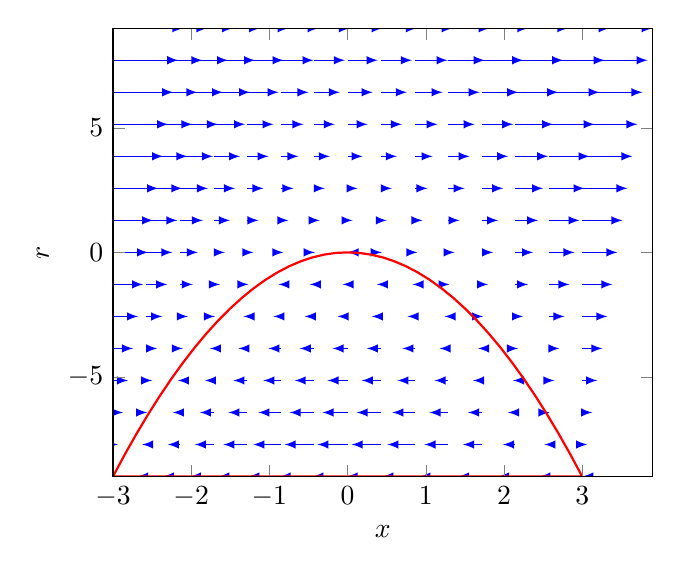
\begin{tikzpicture}
        \begin{axis}[%
         view     = {0}{90}, % for a view 'from above'
         domain   = -3:3,
         y domain = -9:9,
         xlabel = $x$,
         ylabel = $r$,
        %  xtick    = {-3,...,3},
        %  ytick    = {-3,...,3},
       ]
       \addplot3[blue, quiver={u=y+x*x, v=0, w=0, scale arrows=0.05}, samples=15, -latex] (x,y,0);
       \addplot3[red, thick, domain=-3:3, samples=41] ({x},{-x*x},0);
       \end{axis}
    \end{tikzpicture}
\end{center}
where the red line shows the set of fixed points, which we can classify as stable or unstable.
\begin{example}
    Another example is laser threshold operation. How does such a 4-level laser work? We can excite atoms from the ground state to a \textit{pump band} (with a band of energies). These immediately relax into the upper level of the actual laser, which relaxes into the lower level of the laser through the cavity as light, and relaxes back into the ground state.
    \vspace{2mm}

    The upper and lower levels of the laser are curved mirrors and the area between is the cavity. The light inside the cavity is a normal mode of an electromagnetic field. This is a simple harmonic oscillator, so we can quantize it. These levels are described,
    \begin{equation*}
        \ket{n} = \frac{1}{\sqrt{n!}} (a^\dagger)^n \ket{0},
    \end{equation*}
    where $\ket{0}$ is the ground state with energy $\frac{1}{2}\hbar\omega_0.$ The quantum mechanical amplitude $n$ photons in a cavity will produce \textit{another} photon can be calculated,
    \begin{equation*}
        \bra{n+1}|a^\dagger\ket{n} = \sqrt{n+1},
    \end{equation*}
    which shows some sort of positive feedback mechanism. Once the power goes above a certain point $P_\text{cr}$, the laser power output becomes nonzero. This slope is called the slope efficiency.
    \begin{center}
        \begin{tikzpicture}
        \begin{axis}[
        legend pos=outer north east,
        title=Laser Threshold Operation,
        axis lines = box,
        xlabel = $P_\text{lum}\text{ power}$,
        ylabel = $\text{laser power output}$,
        variable = t,
        trig format plots = rad,
        xmin=0,
        xmax=6,
        ]
        \addplot [
            domain=4:6,
            samples=70,
            color=blue,
            ]
            {x-2};
        \addlegendentry{Slope Efficiency}
        \end{axis}
        \end{tikzpicture}
    \end{center}
    Let $n$ be the number of photons, and let 
    \begin{equation*}
        \dot{n} = GnN - kn,
    \end{equation*}
    where $N$ is the number of excited atoms, $k$ represents losses in output photons, and $G$ is the gain cross-section. Note that the excited atoms can be pumped, i.e. via
    \begin{itemize}
        \item an electric discharge (HeNe,CO2,Ar ion lasers)
        \item optical pumping (flashlamp, Nd:glass, Nd:Yag)\footnote{The term after Nd is the host. For example, we can melt Yag and grow a crystal and grow it to contain Nd, which already has a lot of thermal modes which can take away heat}
        \item chemical laser (makes new molecules but are left excited)
    \end{itemize}
    We can describe 
    \begin{equation}
        N(t) = N_0 - \alpha n(t),
    \end{equation}
    where $\alpha$ describes the loss of excited atoms because they were used to amplify the laser and $N_0$ is the number of atoms that have been pumped at the start. Putting everything together,
    \begin{align*}
        \dot{n} &= Gn(N_0 - \alpha n) - kn  \\ 
        &= (GN_0-k)n - (G\alpha)n^2 \\ 
        &= nG\left(N_0 - \frac{K}{G}\right)\left(1 - \frac{\alpha}{N_0 - K/G}n\right).
    \end{align*}
    Compare this to the logistic equation, $\dot{N} = rN\left(1-N/K\right).$ Therefore, the laser will depend on the sign of $N_0-\frac{K}{G}.$ Therefore, depending on how much we pump the laser, we can change the qualitative behavior. Consider the following cases,
    \begin{itemize}
        \item Weak pumping, $N_0 < K/G.$ This implies that $n=0$ is the only fixed point. The steady state dynamic is the case where nothing happens, so it goes to $n=0.$
        \item Strong pumping, $N_0 > K/G.$ We gain a new stable fixed point, and moved off the origin $n=0.$ The hold fixed point now becomes unstable.
    \end{itemize}
    The bifurcation diagram is,
    \begin{center}
        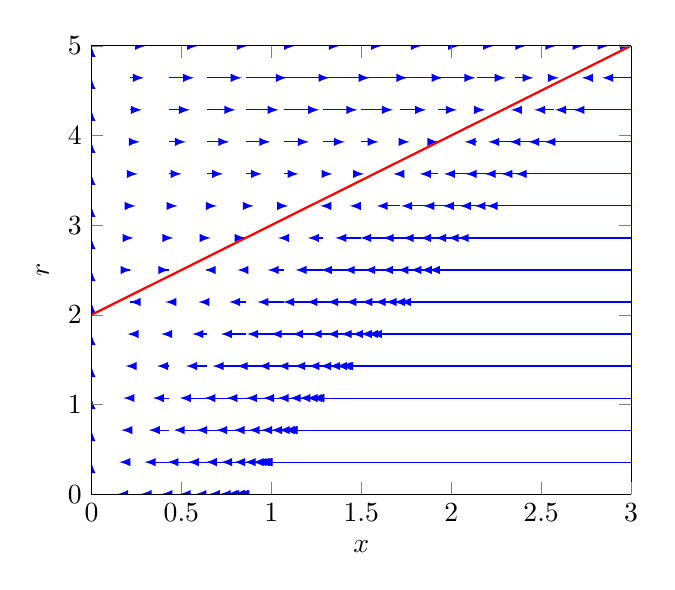
\begin{tikzpicture}
            \begin{axis}[%
             view     = {0}{90}, % for a view 'from above'
             domain   = 0:3,
             y domain = 0:5,
             xlabel = $x$,
             ylabel = $r$,
            %  xtick    = {-3,...,3},
            %  ytick    = {-3,...,3},
           ]
           \addplot3[blue, quiver={u=3*x*(y-2)*1-x*3*x, v=0, w=0, scale arrows=0.05}, samples=15, -latex] (x,y,0);
            \addplot3[red, thick, domain=0:3, samples=41] ({x},{x+2},0);
           \end{axis}
        \end{tikzpicture}
    \end{center}
\end{example}
There are different types of bifurcations,
\begin{itemize}
    \item Saddle-node:
    \item Transcritical:
    \item Pitchfork: This is caused when a change in parameter can cause a fixed point to branch out into three directions. Some examples,
    \begin{itemize}
        \item \textit{Phase transitions}: As water vapour condenses to water, it gives up a lot of heat. This is the reason behind hurricanes. As vapour condenses, the heat it gives up heats the surrounding air, creating strong convection currents, causing more and more water droplets through a positive feedback loop.
        \item Magnetic spin systems, higgs phenomena, QCD
    \end{itemize}
    This bifurcation applies to system possessing $Z_2$ symmetry. That is,
    \begin{equation*}
        \sigma: x \mapsto -x,
    \end{equation*}
    so $\sigma^2 \equiv 1.$ Now consider the equation
    \begin{equation*}
        \dot{x} = rx-x^3,
    \end{equation*}
    which is the normal form for a \emf{supercritical pitchfork bifurcation.} The roots are,
    \begin{equation*}
        x=0,\pm\sqrt{r},
    \end{equation*}
    where $\pm\sqrt{r}$ exists and are distinct only for $r>0.$ For $r<0,$ we have $x=0$ as the only fixed point.
    \begin{center}
        \begin{tikzpicture}
        \begin{axis}[
        legend pos=outer north east,
        title=Pitchfork Bifurcation,
        axis lines = middle,
        xlabel = $r$,
        ylabel = $x^*$,
        variable = t,
        trig format plots = rad,
        ]
        \addplot [
            domain=-4:0,
            samples=70,
            color=blue,
            ]
            {0};
        \addplot [
            domain=0:4,
            samples=70,
            color=blue,
            ]
            {sqrt(x)};
        \addplot [
            domain=0:4,
            samples=70,
            color=blue,
            ]
            {-sqrt(x)};
            \draw [blue,-, dashed, ultra thick] (axis cs:0,0) -- (axis cs:4,0);
        \end{axis}
        \end{tikzpicture}
    \end{center}
    Consider
    \begin{equation*}
        \dot{x}=rx+x^3-x^5,
    \end{equation*}
    which is a \emf{subcritical pitchfork bifurcation.} These correspond to a 1st order phase transition and supercritical bifurcations correspond to 2nd order phase transitions.

    The reason that 2nd order phase transitions are smooth because when fixed points are created, they are created from the origin. But for 1st order phase transitions, as we transition from stable to unstable, \textit{before} the system becomes unstable, new (stable) fixed points can be created and when the $x=0$ solution becomes unstable, the stable solutions make a sudden jump.
\end{itemize}
\subsection{Ising Model}
Suppose we have a $Z_2$ system with 2 spins and our model is in $d$-dimensional space and each electron is on the vertex of a lattice with values $\pm 1.$ There is no fundamental difference between the up and down state, i.e. the energy.

Assume there is no external magnetic field, so we only have relationships between spins. Assume only nearest neighbours interact. There are two possibilities,
\begin{itemize}
    \item If $\uparrow\uparrow$ is lowest energy, this is ferromagnetic
    \item If $\uparrow\downarrow$ is lowest energy, it is antiferromagnetic.
\end{itemize}
We work with ferromagnetics for now. The Hamiltonian is
\begin{equation*}
    \mathcal{H} = \text{energy of spin-system} = -|J| \sum_{\langle i,j\rangle} s_i s_j + h\sum_i s_i,
\end{equation*}
where the first term is $Z_2,$ but the 2nd term introduces a bias/preference/asymmetry and is no longer $Z_2.$

We now introduce a macroscopic quantity
\begin{equation*}
    M \equiv \sum_{i=1}^N s_i
\end{equation*}
is the total/net spin. Here, $M$ is an example of an \emf{order parameter,} with $M=N$ meaning all up and $M=-N$ meaning all down. The Ising model looks at the symmetric case where $h=0$ and $d=2,3.$

For curie temperatures greater than $T>T_C,$ we have $\langle M \rangle = 0,$ but if $T<T_C,$ we have $\langle M \rangle \neq 0$ and there is now a preffered direction 

In this phase where symmetry is spontaneously broken ($T<T_c$), it is unstable to have equal numbers $\uparrow,\downarrow.$
\section{Two-Dimensional Equations}
For a 2d nonlinear equation, we can find fixed points and linearize there to analyze stability, i.e. a matrix with constant entries. If the matrix for the system can be diagonalized, then we decouple $x,y$ so the evolution of $x'$ only depends on $x,$ and similarly for $y'.$ There are different cases,
\begin{itemize}
    \item $\lambda_1,\lambda_2>0$ gives unstable nods
    \item $\lambda_1,\lambda_2<0$ gives stable nodes
    \item $\lambda_1>0,\lambda_2<0$ gives saddle nodes
\end{itemize}
But what if it's not diagonalizable in $\mathbb{R}^2?$ Suppose we have the rotation matrix for a $90^\circ$ rotation, which gives us 
\begin{equation*}
    \begin{pmatrix}
        \dot{x} \\ \dot{y}
    \end{pmatrix} = \begin{pmatrix}
        0 & -1 \\ 
        1 & 0
    \end{pmatrix}\begin{pmatrix}
        x\\y 
    \end{pmatrix}.
\end{equation*}
While this can't be diagonalized, it represents a vector field that can be integrated in circles. In the phase space for $(x,\dot{x}),$ we have concentric circles, which is also true for simple harmonic oscillators. We can analyze in general,
\begin{itemize}
    \item Case 1: Both roots are related
    \begin{itemize}
        \item Case 1a: $(\tr A)^2 \ge 4 \det A$ We have distinct eigenvalues, and get nodes with the sign (stable/unstable) or saddle nodes with mixed signs.
        \item Case 1b: $(\tr A)^2 = 4 \det A$ We have repeated eigenvalues, and get two equal valued eigenvalues 
        \begin{equation*}
            \lambda_1=\lambda_2 = \frac{\tr A}{2}.
        \end{equation*}
        \begin{itemize}
            \item Case 1b(i): $A$ is symmetric $A=A^T.$ Then we have a star shape.
            \item Case 1b(ii): $A$ is not symmetric. We have only a single eigenvector,
            \begin{equation*}
                v_2=\begin{pmatrix}
                    (a-b)/2d \\ 1
                \end{pmatrix}.
            \end{equation*}
            This can be thought of as the limiting case of two nearly parallel eigenvectors.
        \end{itemize}
    \end{itemize}
\end{itemize}
\end{document}